\laborator{Основы математического пакета Mathcad}

\goal ознакомиться с пользовательским интерфейсом математического пакета Mathcad; изучить способы задания различного типа переменных и функций; освоить приемы работы с графическим и текстовым редакторам; ознакомится с процедурами численного решения алгебраических уравнений и систем уравнений, реализованными в данном пакете.

Mathcad --- программное средство, являющееся средой для выполнения на компьютере разнообразных расчетов. Mathcad включает в свой состав три редактора --- формульный (по умолчанию), текстовый и графический. Благодаря им обеспечивается принятый в математике способ записи функций и выражений и получение результатов вычислений, произведенных компьютером в виде таблиц и графиков. Взаимодействие пользователя с компьютером осуществляется с помощью удобного графического интерфейса, включающего пиктограммы, диалоговые окна, меню, опции и другие «инструменты», располагаемые на экране дисплея. Mathcad включает множество операторов, встроенных функций и алгоритмов решения разнообразных математических задач.

Пользовательский интерфейс системы создан так, что пользователь, имеющий элементарные навыки работы с Windows~- приложениями, может сразу начать работу с Mathcad. Работа с документами Mathcad обычно не требует обязательного использования возможностей главного меню, так как основные из них дублируются пиктограммами управления. Пиктограммы управления представляют собой перемещаемые наборные панели, которые содержат заготовки из шаблонов математических знаков (цифр, знаков арифметических операций, матриц, знаков интегралов, производных и т.д.). Наборные панели могут быть выведены на экран все сразу или в нужном количестве. Кнопки на наборных панелях вводят в месте расположения курсора общепринятые и специальные математические знаки и операторы. На рис. \ref{fig:oldmathcad.view} представлены наборные панели Mathcad, вызываемые из панели инструментов «Математическая» (\menu[,]{Вид, Панель инструментов, Математическая}) :
\begin{itemize}
\item Калькулятор --- содержит арифметические инструменты;
\item Графики --- содержит инструменты графиков;
\item Матрицы --- содержит векторные и матричные операции;
\item Вычисления --- содержит инструменты вычислений;
\item Высшая математика --- содержит операторы математического анализа;
\item Булева алгебра --- содержит инструменты булевой алгебры;
\item Программирование --- содержит инструменты программирования;
\item Греческий алфавит – содержит символы греческого алфавита;
\item Символьно --- содержит символьные операторы.
\end{itemize}

\begin{figure}[h]
	\begin{center}
		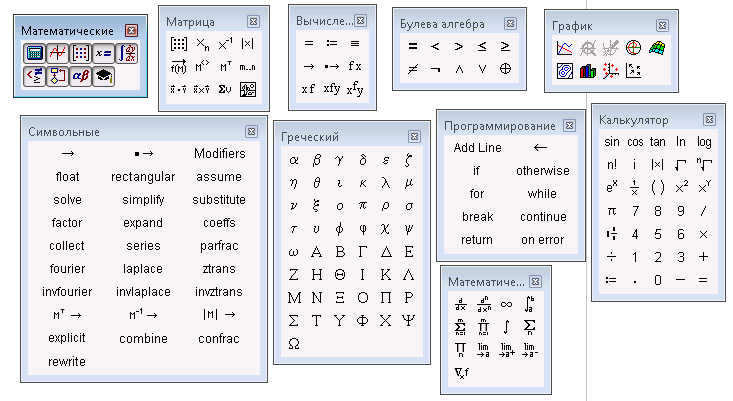
\includegraphics[width=\textwidth]{oldview.png}
	\end{center}
	\caption{Наборные панели пакета Mathcad} \label{fig:oldmathcad.view}
\end{figure}

По умолчанию ввод осуществляется в вычислительный блок. Для запуска формульного редактора достаточно установить курсор мыши в любом свободном месте окна редактирования и щелкнуть левой клавишей. Появится визир в виде маленького красного крестика. Его можно перемещать клавишами перемещения курсора. Визир указывает место, с которого можно начинать набор формул --- вычислительных блоков. Подготовка вычислительных блоков облегчается благодаря выводу шаблона при задании того или иного оператора при помощи наборных панелей (см. рис. \ref{fig:oldmathcad.view}). Для ввода данных можно указать курсором мыши на нужный шаблон данных и щелчком левой ее клавиши ввести его.

Чтобы определить переменную, необходимо выполнить следующие действия:
\begin{itemize}
	\item набрать имя переменной (регистр имеет значение);
	\item ввести оператор присваивания «:=», сделать это можно нажатием кнопки «Определение» панели «Калькулятор» или «Вычисления» либо с помощью сочетания клавиш \keys{\shift+:};
	\item на место черного маркера, появившегося справа от оператора присваивания, ввести значение переменной.
\end{itemize}
Mathcad позволяет работать со следующими типами переменных:
\begin{itemize}
\item скалярная величина;
\item вектор (который также может быть задан с помощью оператора ранжированной переменной);
\item матрица.
\end{itemize}

Если переменная определяется как скалярная величина, то ее численное значение вводится с клавиатуры на место черного маркера. Работа в Mathcad осуществляется аналогично программированию на языках интерпретаторах, т.е. программа выполняется слева направо и сверху вниз. Это означает, что переменные должны быть определены в тексте программы левее или выше места их использования.

\primer{Используя формульный редактор, задайте переменную \mc{Data}, присвойте ей значение, целая часть которого --- день вашего рождения, десятичная --- месяц (например 1 января), и распечатайте ее экране используя оператор числового вычисления «=» на панели «Калькулятор»}
	\begin{center}
		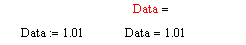
\includegraphics{oldz1.png}
	\end{center}

Если распечатать переменную \mc{Data} левее и выше ее места определения, то Mathcad выдаст ошибку.

\subsubsection*{Текстовый редактор}
Текстовый режим в Mathcad позволяет создавать всевозможные комментарии и качественно оформлять решенные задачи.
Чтобы ввести текстовую область, нажмите сочетание клавиш \keys{\shift+ ‘} (курсор ввода при этом должен располагаться на чистом участке документа). При этом появится специальная рамка, а курсор ввода приобретет вид красной вертикальной линии.
Набирается текст в Mathcad точно так же, как в любом текстовом редакторе. Если известно, сколько места на листе займет комментарий, то можно сразу растянуть текстовую область до нужных размеров. Чаще же текст просто вводят в область, обрывая строки с помощью клавиши \keys{\enter}, когда они достигают нужной длины (это приходится делать, так как Mathcad не выполняет автоматически переносов слов).

\primer{Сделайте шапку для документа: введя название лабораторной работы, номер группы и фамилию с инициалами:}
\begin{center}
	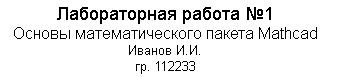
\includegraphics{oldz2.png}
\end{center}


\subsubsection{Массивы (векторы, матрицы)}
Массивы, по принципу задания их элементов, можно разделить на две группы:
\begin{itemize}
	\item векторы и матрицы, при задании которых не существует прямой связи между величиной элемента и его индексами;
	\item ранжированные переменные --- векторы, величина элементов которых напрямую определяется индексом.
\end{itemize}
В Mathcad реализовано несколько способов задания массивов:
\begin{itemize}
	\item задание матрицы или вектора вручную с помощью команды «Вставить матрицу»;
	\item определение матрицы последовательным заданием каждого элемента;
	\item  использование ранжированных переменных;
	\item создание таблицы данных;
	\item чтение из внешнего файла, и др.
\end{itemize}

Наиболее простым способом задания матрицы является использование специального окна «Вставить матрицу» (вызывается нажатием кнопки «Матрица или вектор» на наборной панели «Матрицы» или сочетанием клавиш \keys{\ctrl+M}). Параметры создаваемой матрицы или вектора можно определить в окошках «Строк» и «Столбцов». В результате в документ будет вставлена заготовка с черными маркерами вместо элементов, в которые необходимо ввести нужные значения:

\begin{center}
	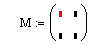
\includegraphics{oldz3-m.png}
\end{center}


Элементы матрицы могут быть как числами, так и выражениями. Если среди выражений или символов, выступающих в качестве элементов матрицы, есть неизвестные или параметры, то они обязательно должны быть численно определены выше. В противном случае матрица должна быть задана как функция.

\primer{Задайте вектор \mc{B}, содержащий три произвольных численных значения, и квадратную матрицу \mc{M}, содержащую девять произвольных значений, и распечатайте их:}

\begin{center}
	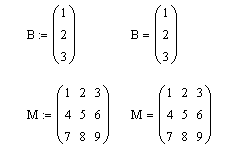
\includegraphics{oldz3.png}
\end{center}


В случае заданной матрицы всегда можно получить значение любого его элемента, используя его матричные индексы. Матричные индексы равняются номеру строки и столбца, на пересечении которых элемент находится. В математике отсчет строк и столбцов принято начинать с единицы. В программировании же начальные индексы обычно равняются нулю. По умолчанию в Mathcad строки и столбцы тоже начинаются с нуля. В том случае если такая система не удобна, то точку отсчета можно изменить на вкладке «Опции рабочего листа» (вкладка основного меню «Инструменты») изменив параметр «Начальный индекс» на единицу.

Итак, чтобы получить значение какого-то матричного элемента, нужно ввести имя матрицы с соответствующими индексами и поставить «=». Для задания индексов на панели «Матрицы» имеется специальная кнопка «Нижний индекс», которой соответствует клавиша \keys{[} . Нажав ее, вы увидите, что на месте будущего индекса, чуть ниже текста имени матрицы, появится черный маркер . В него через запятую следует ввести значения индексов. На первом месте при этом должен стоять номер строки, а на втором – номер столбца. При выделении элемента вектора нужно задать только индекс строки. Индексы также могут быть определены и через выражения или специальные функции.

Помимо одного элемента можно очень просто выделить и целые матричные столбцы. Чтобы это сделать, нужно использовать специальный оператор панели «Матрицы» «Столбец матрицы» (также вводится сочетанием  \keys{\ctrl + 6})  и в черный маркер ввести требуемый номер столбца. В том случае, если требуется выделить строку, матрицу необходимо транспонировать (оператор «Транспонирование матрицы» той же рабочей панели).

\primer{Обратитесь к центральному элементу матрицы М и распечатайте его значение. Обратитесь к первому столбцу матрицы М и распечатайте его значение. Обратитесь к второму элементу вектора В и распечатайте его значение. Измените начало отсчета векторов и матриц с 0 на 1 и повторите задание:}

\begin{center}
	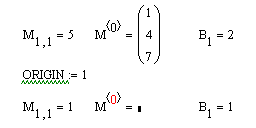
\includegraphics{oldz3-2.png}
\end{center}


При работе с массивами Mathcad воспринимает их как матрицы, поэтому при вычислениях будут применяться матричные операции (сложение, умножение и т.д.). Однако зачастую при расчетах матрицы используются для хранения однотипных данных, зависимостей. Поэтому в вычислениях необходимо использовать поэлементные операции, когда операции производятся над элементами с соответствующими индексами. Для осуществления поэлементных матричных операций на панели  «Матрица» есть кнопка векторизовать  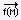
\includegraphics{oldz3-3.png}(сочетание клавиш \keys{\ctrl + -})

\primer{Задайте две квадратные матрицы \mc{A} и \mc{B} с произвольными значениями элементов. Найдите произведение матриц и поэлементное произведение элементов:}

\begin{center}
	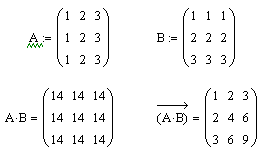
\includegraphics{oldz3-4.png}
\end{center}


\subsubsection*{Ранжированные переменные}
Одной из разновидностей задания массивов является использование так называемых ранжированных переменных. Ранжированная переменная – это разновидность вектора, особенностью которого является непосредственная связь между индексом элемента и его величиной. В Mathcad ранжированные переменные очень активно используются как аналог программных операторов цикла (например, при построении графиков).
Простейшим примером ранжированной переменной является вектор, значение элементов которого совпадает с их индексами. Для задания такой ранжированной переменной выполните следующую последовательность действий.
\begin{enumerate}
	\item Введите имя переменной и оператор присваивания.
	\item  Поставив курсор в маркер значения переменной, нажмите кнопку «Диапазон переменных» панели «Матрицы». При этом будет введена заготовка в виде двух маркеров, разделенных точками:
	\begin{center}
		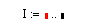
\includegraphics{oldz4-1.png}
	\end{center}
		
	Данную заготовку можно вставить с помощью клавиши \keys{;}.
	
	\item  В левый черный маркер заготовки ранжированной переменной введите ее первое значение, в правый – последнее.
\end{enumerate}

Шаг изменения ранжированной переменной при ее задании с помощью описанного способа постоянен и равен единице. Однако при необходимости его можно сделать и произвольным. Дли этого нужно, поставив после левой границы интервала запятую, ввести второе значение ранжированной переменной. Разность между первым и вторым ее значением и определит шаг. 
Использование ранжированных переменных во многом основано на том, что большинство математических действий в Mathcad над векторами осуществляется точно так же, как над простыми числами. Так, например, существует возможность вычисления значений практически любой встроенной и пользовательской функции от вектора. При этом в качестве результата будет выдан вектор, составленный из значений функции при величинах переменных, равных соответствующим элементам исходного вектора.

\primer{Задайте ранжированную переменную \mc{С} от 0 до 3 (шаг изменения переменной по умолчанию) и распечатайте ее значения. После задайте новый шаг изменения ранжированной переменной \mc{Е} (например 0.5) и распечатайте ее значения:}
\begin{center}
	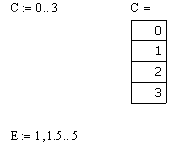
\includegraphics{oldz4-2.png}
\end{center}

\subsubsection*{Таблицы}
Все экспериментальные данные обрабатываются в Mathcad в виде матриц. Однако использовать описанные выше стандартные методы задания массивов для этого крайне неудобно. В этом случае можно использовать так называемую таблицу ввода. Чтобы ее вызвать, задействуйте команду \menu[,]{Вставить, Данные, Таблица} главного меню (соответствующая этой команде кнопка имеется и на панели «Стандартные»). В документ будет введена следующая заготовка:
\begin{figure}[h]
	\begin{center}
		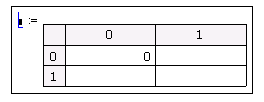
\includegraphics{oldz5-1.png}
	\end{center}
\end{figure}

Присвоив будущей матрице определенное имя (вводится в черный маркер слева от знака присваивания), попробуйте определиться с ее размерами. Если она не очень большая, можно сразу расширить пустую таблицу до нужной величины. Для этого следует использовать специальные черные маркеры, появляющиеся на контуре таблицы при ее выделении. Никаких ограничений на размеры таблица ввода не имеет. Создание таблицы повторяет заполнение обычных матриц, однако в таблицах нельзя использовать формулы.

Так как таблицы являются для Mathcad такими же матрицами, как заданные стандартными способами, с ними можно проводить все те же преобразования, что и со стандартными массивами. Если отобразить содержание таблицы через ее имя, оно визуализируется (при стандартных настройках) как простая матрица.

\primer{Задайте таблицу \mc{Т}, состоящую из 2 столбцов и 5 строк (нумерацию массивов начать с 0). Распечатать отдельно каждый столбец таблицы и один из элементов таблицы:}
\begin{figure}[h]
	\begin{center}
		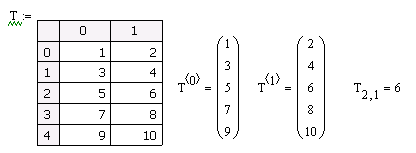
\includegraphics{oldz5-2.png}
	\end{center}
\end{figure}


\subsubsection{Операторы}
Операторы --- это символ или последовательность символов, обозначающих то или иное математическое действие. Операторы, выполняющие все основные арифметические действия, расположены на панели «Калькулятор» (рис. \ref{fig:oldmathcad.view}). Ввод основных арифметических операторов может быть также осуществлен с клавиатуры.

\subsubsection{Функции}
Функции в Mathcad делятся на две группы:
\begin{itemize}
\item функции пользователя;
\item встроенные функции.
\end{itemize}
Техника использования функций обоих типов абсолютно идентична, а вот задание отличается принципиально. Для задания функции пользователя необходимо выполнить следующие действия:
\begin{itemize}
\item ввести имя функции;
\item после имени ввести пару круглых скобок, в которых через запятую необходимо указать все переменные, от которых зависит функция;
\item ввести оператор присваивания «:=»;
\item на место черного маркера, появившегося справа от оператора присваивания, необходимо задать вид функции.
\end{itemize}

В выражение определяемой функции могут входить как непосредственно переменные, так и другие встроенные и пользовательские функции. 

Встроенные функции --- это функции, заданные в Mathcad изначально. Чтобы их использовать, достаточно корректно набрать имена функций с клавиатуры. Наиболее распространенные из них можно ввести с панели «Калькулятор», это синус, косинус, тангенс, натуральный и десятичный логарифмы, экспонента. Для того чтобы задать все остальные встроенные функций Mathcad, нужно открыть специальное окно «Вставить функции».

\primer{ Задайте пользовательскую функцию $y=x^2+x-1$, подставьте в качестве аргумента ранее определенные переменные \mc{Data} и \mc{С}, а также выражение \mc{2 Data}:}
\begin{figure}[h]
	\begin{center}
		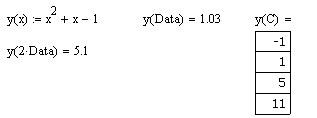
\includegraphics{oldz6-1.png}
	\end{center}
\end{figure}

\primer{Задайте пользовательскую функцию $y(x)=\dfrac{x^2 +\cos(x)}{2}$, 
подставьте в качестве аргумента ранее определенные переменные \mc{Date} и \mc{С}:}
\begin{figure}[h]
	\begin{center}
		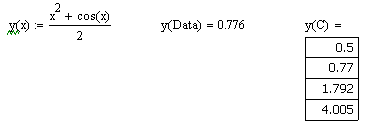
\includegraphics{oldz6-2.png}
	\end{center}
\end{figure}

\subsubsection{Графический редактор}
Все основные типы графиков и инструменты работы с ними расположены на рабочей панели «Графики» (рис. \ref{fig:oldmathcad.view}). Здесь можно найти ссылки на семь типов графиков. В курсе математического моделирования потребуются только график кривой в двумерной декартовой системе координат. Соответствующая графическая заготовка вызывается из наборной панели «Графики» -Y график 
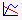
\includegraphics{oldz7-1.png}:
\begin{figure}[h]
	\begin{center}
		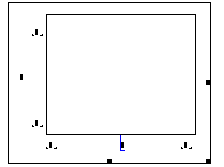
\includegraphics{oldz7-2.png}
	\end{center}
\end{figure}

На рисунке область ввода значения аргумента и функции обозначена черными метками по центру соответствующих осей. По оси абсцисс откладывается аргумент, например \mc{x}, по оси ординат функция -- например \mc{y(x)}. Границы по осям выставляются автоматически, но предусмотрено их изменение вручную. Переход к редактированию осуществляется постановкой курсора в соответствующий регистр по осям абсцисс и ординат, на рисунке это черные метки в начале и конце каждой оси, отмеченные по краям снизу черными угловыми линиями.

В ряде случаев (например, если в графике приходится очень часто менять диапазоны по осям или необходимо выделить конкретную область) можно задать векторы данных самостоятельно. Сделать это можно с помощью оператора ранжированной переменной (задание ранжированной переменной рассматривалось выше). В этом случае аргумент функции задается в виде вектора, т.е. переменная и функция будут заданы в виде двух соразмерных векторов, по которым будет построен график.

Mathcad позволяет отображать до 16 графических зависимостей в одной системе координат, что удобно для визуального контроля и сравнения полученных результатов. Чтобы добавить к уже имеющемуся графику еще один, выполните следующую последовательность действий:
\begin{itemize}
	\item Установите курсор справа от выражения, определяющего координаты последнего ряда данных по оси \mc{y} (предварительно выделив его).
	\item Нажмите клавишу \keys{,}. При этом курсор опустится на строку ниже и появится чистый маркер.
	\item В появившийся маркер введите выражение для новой функции или имя функции.
\end{itemize}

С помощью описанного метода можно построить графики функций одной переменной. Если же кривые, которые нужно отобразить на одной области, зависят от различных переменных, то их, аналогично добавлению новых функций, следует ввести через запятую в нижний маркер в том же порядке, что и соответствующие им функции.

Изменение настроек отображения осей и графиков (если необходимо изменить тип или цвет кривой) осуществляется с помощью диалогового окна «Форматирование выбранной декартовой плоскости», вызвать которое можно, дважды щелкнув левой кнопкой мыши на области графика.

\primer{Постройте графическую зависимость для функции \mc{y(x)}, определенной в предыдущем задании и функции $5 \sin(x)$. Измените диапазон графика путем определения аргумента как ранжированной переменной от 0 до 5. Посмотрите как шаг ранжированной переменной влияет на график:}

\begin{center}
	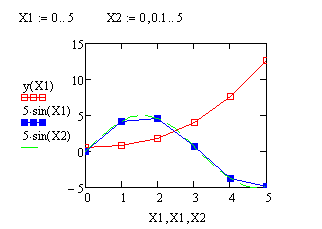
\includegraphics{oldz8-1.png}
\end{center}


\subsubsection*{Символьные вычисления}
В Mathcad имеет возможности символьных вычислений: решение уравнений, преобразования, разложения и т.д. Для аналитического преобразования можно воспользоваться кнопкой 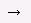
\includegraphics{oldz11-1.png} на панели «Символьные вычисления» или сочетанием \keys{\ctrl + .}
\primer{Вычислите производную и интеграл выражения $x^2+\sin(x)$}
%\begin{figure}[h]
	\begin{center}
		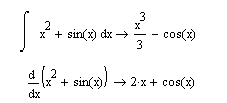
\includegraphics{oldz11-2.png}
	\end{center}
%\end{figure}

\subsubsection*{Численное решение уравнений и систем уравнений}
Для численного поиска решений уравнений с одним неизвестным в Mathcad существует специальная встроенная функция \mc{root}. Функция эта может использоваться в двух различных формах, при этом реализуются разные численные алгоритмы. Так, если определена только одна точка приближения к корню, поиск решений будет осуществляться методом секущих. Если же задан интервал, на котором предположительно локализовано решение, то поиск его будет осуществлен с применением двух модификаций метода бисекции.

Если необходимо найти корень некоторого уравнения, причем известен интервал, в котором он локализован, проще всего использовать функцию с четырьмя аргументами: \mc{rоot(f(x), x, a, b)}, где \mc{f(x)} --- функция, определяющая уравнение, \mc{х} --- переменная, \mc{a} и \mc{b} --- границы интервала локализации. Обязательным условием является то, что значения функции на концах интервала должны быть противоположных знаков. Это связано с особенностью используемых \mc{root} алгоритмов. Если нарушить это условие, система выдаст сообщение об ошибке.


В тех случаях, когда определить границы такой локализации невозможно, следует применять функцию \mc{root} с одной точкой приближения: \mc{rоot(f(x),x)}. В этом случае необходимо перед вызовом функцию \mc{root} задать для переменной \mc{x} начальное приближение.

Важной характеристикой решения является его точность. В Mathcad можно регулировать величину погрешности решения, изменяя значение специальной системной переменной \mc{TOL}. В общем случае, чем меньше \mc{TOL}, тем точнее будет найден корень, но и тем больше времени уйдет на его определение (а также будет выше риск, что численный метод не сойдется к решению).

\primer{Найти с помощью функции \mc{root} корни уравнения: $x^3-10 x +2 =0$
	используя различные интервалы локализации и точки начального приближения:}
\begin{figure}[h]
	\begin{center}
		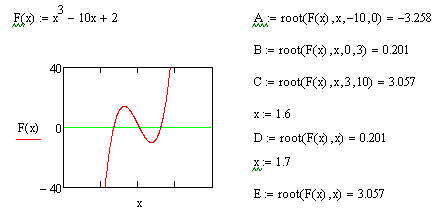
\includegraphics{oldz9-1.png}
	\end{center}
\end{figure}

Для численного решения систем уравнений в Mathcad служит блок \mc{Given-Find}. Используя блок \mc{Given-Find}, можно решать системы, содержащие до 250 нелинейных уравнений и до 1000 линейных. Результатом решения системы будет численное значение искомых корней.


Для решения системы уравнений с помощью блока \mc{Given - Find} необходимо выполнить следующее:
\begin{itemize}
	\item Задайте начальные приближения для всех неизвестных, входящих в систему уравнений. Mathcad решает уравнения при помощи итерационных методов. На основе начального приближения строится последовательность, сходящаяся к искомому решению. 
	\item Напечатайте в рабочем окне Mathcad ключевое слово \mc{Given}. Оно указывает Mathcad, что далее следует система уравнений.
	\item Введите уравнения и неравенства в любом порядке ниже ключевого слова \mc{Given}. В качестве знаков равенства следует использовать логическое равенство . Ввести его можно нажатием кнопки «Булево равенство» панели «Булева алгебра» либо с помощью сочетания клавиш \keys{\ctrl+ =}. Между левыми и правыми частями неравенств может стоять любой из логических символов $<$, $>$, $\leqslant$ и $\geqslant$ (панель «Булева алгебра»).
	\item Введите функцию решения систем уравнений \mc{Find}{$\mathrm{(x_1, x_2)}$} и оператор численного вывода (знак «=»). В скобках через запятую задайте переменные в том порядке, в котором должны быть расположены в ответе соответствующие им корни. Если результаты решения требуется использовать в дальнейших расчетах, то тогда их необходимо присвоить некоторой переменной \mc{Z:=Find}{$\mathrm{(x_1, x_2)}$}.
\end{itemize}

\primer{Решите систему нелинейных уравнений $\sqrt{x}+\sqrt{y}=9$, и $\sqrt[3]{x}+ \sqrt[3]{y}=5$ выведите результат на печать:}

\begin{center}
	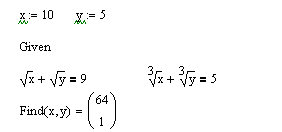
\includegraphics{oldz9-2.png}
\end{center}

Вопросы для самоконтроля
\begin{enumerate}
	\item Для каких целей предназначен математический пакет Mathcad?
	\item С какими типами переменных позволяет работать Mathcad?
	\item В чем разница между оператором присваивания и оператором численного решения?
	\item Какие типы функций есть в Mathcad, в чем их отличие?
	\item  Для чего предназначен графический редактор?
	\item Для чего предназначен текстовый редактор?
\end{enumerate}